\fontsize{13}{14}\selectfont
\section{PROCEDURE}

\subsection{Load data}

\begin{lstlisting}[style=StyleCode, language=MATLAB]
	% Clear the workspace
	clear;
	% Load the user_movies.mat file
	load('users_movies.mat', 'movies', 'users_movies', 'users_movies_sort', 'index_small', 'trial_user')
\end{lstlisting}

First, we load the data from the file “\texttt{users\_movies.mat}” using the “\texttt{load}” command. "\texttt{load}" helps us to load actual data stored in those variables shown below while "\texttt{clear}" is used to clear all variables in MATLAB workspace to ensure that no old data interferes. The matrix “\texttt{users\_movies}” should have dimensions $6040 \times 3952$, with integer values ranging from 0 to 5. A rating of 1 represents “strongly dislike”, while 5 represents “strongly like”. A rating of 0 indicates that the user did not rate the movie. The array “movies” contains the titles of all the movies. Moreover, the matrix “users movies sort” is a subset of “\texttt{users\_movies}”, containing ratings for the 20 most popular movies.

\begin{center}
	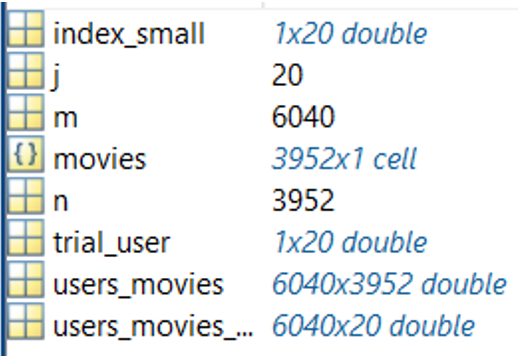
\includegraphics[width=.3\linewidth]{sections/pic/section3/1.png}
\end{center}

Also, the indexes of these popular movies are stored in the array “\texttt{index\_small}”. Finally, the vector “\texttt{trial\_user}” contains ratings of these popular movies by another user who is not part of the database. It is recommended to view all variables and their dimensions using the “Workspace” window in the MATLAB environment.

\subsection{Print the titles}

The figure below shows the 20 most popular movies:

\begin{lstlisting}[style=StyleResult]
	The rating is determined based on the 20 most popular movies:
	1. E.T. the Extra-Terrestrial (1982)
	2. Star Wars Episode IV - A New Hope (1977)
	3. Star Wars Episode V - The Empire Strikes Back (1980)
	4. Star Wars Episode VI - Return of the Jedi (1983)
	5. Jurassic Park (1993)
	6. Saving Private Ryan (1998)
	7. Terminator 2: Judgment Day (1991)
	8. The Matrix (1999)
	9. Back to the Future (1985)
	10. The Silence of the Lambs (1991)
	11. Star Wars Episode I - The Phantom Menace (1999)
	12. Raiders of the Lost Ark (1981)
	13. Fargo (1996)
	14. The Sixth Sense (1999)
	15. Braveheart (1995)
	16. Shakespeare in Love (1998)
	17. The Princess Bride (1987)
	18. Schindler's List (1993)
	19. The Shawshank Redemption (1994)
	20. Groundhog Day (1993)
\end{lstlisting}

The code below is use to print top 20 most popular movies.

\begin{lstlisting}[style=StyleCode, language=MATLAB]
	% Get the dimensions
	[m, n] = size(users_movies);
	
	% Print a header indicating the movies to be listed
	fprintf('The rating is determined based on the %d most popular movies: \n', length(index_small))
	
	% Loop through of the popular movies
	for j = 1:length(index_small)
		% print the movies title correponding to the current index
		fprintf('%d. %s \n', j, movies(index_small(j)));
	end
	fprintf('\n);
\end{lstlisting}

The "\texttt{fprintf()}" function is a versatile tool used to display formatted text directly in the Command Window. When constructing the output string, special format specifiers are used to indicate how different types of data should be displayed. For instance, "\texttt{\%d}" serves as a placeholder that allows for the printing of an integer value. To control the layout of the output, the newline character, represented as "\texttt{\textbackslash n}", is used to move the cursor to the beginning of the next line, effectively adding a line break.

Generally, "\texttt{length(index\_small)}" is used to determine the total number of elements within an array named "\texttt{index\_small}". This numerical result can then be incorporated into a formatted string using "\texttt{fprintf()}" and the "\texttt{\%d}" specifier to display this count.

Loops are fundamental for repetitive tasks, and the "\texttt{for}" loop is commonly used to execute a block of code multiple times. Within such a loop, “\texttt{fprintf()}” can be employed again to print details for each iteration.

For example, the format string "\texttt{\%d. \%s \textbackslash n}" instructs the program to print an integer (using \texttt{\%d}), followed by a period and a space, then a string of characters (using \texttt{\%s}), and finally, to add a new blank line (\texttt{\textbackslash n}). In short:

\begin{itemize}[label=-]
	\item \textbf{\texttt{\%d}:} Prints the index interger.
	\item \textbf{\texttt{\%s}:} Prints the title movies.
	\item \textbf{\texttt{\textbackslash n}:} Adds new blank line.
\end{itemize}

This is useful for creating numbered lists, such as displaying an index number alongside a movie title. To further improve the visual separation and readability of the output, an additional "\texttt{{fprintf('\textbackslash n')}}" can be used to print an extra blank line, creating better spacing in the Command Window.

\subsection{Select people}

The following code selects people who rated all of the 20 movies under consideration:

\begin{lstlisting}[style=StyleCode, language=MATLAB]
	% Select the users to compare to 
	[m1, n1] = size(users_movies_sort);
	rating = [];
	for j = 1:m1
		if prod(users_movies_sort(j, :)) ~= 0
			rating = [rating; users_movies_sort(j, :)];
		end;
	end;
\end{lstlisting}

\textbf{Explain:}

Initially, the code determines the dimensions of a matrix named "\texttt{users\_movies\_sort}" by using the "\texttt{size()}" function. This function call assigns the number of rows (representing users) to the variable m1 and the number of columns (representing movies) to \texttt{n1}. Following this, an empty matrix called ratings is created, which will be used to store selected user data:

\begin{itemize}[label=-]
	\item \texttt{[m1, n1] = size(users\_movies\_sort)}: Measure the size of the users\_movies\_sort matrix. m1 is the number of users (rows), n1 is the number of movies (columns).
	\item \texttt{ratings = []}: Create an empty matrix called ratings.
\end{itemize}

The core of this code segment is a for loop that iterates through each user, from the first user (index 1) up to m1 (the total number of users). Inside this loop, a conditional check is performed using an if statement. This condition evaluates the product of all ratings for the current user \texttt{j} (accessed via \texttt{users\_movies\_sort(j, :)}). If this product is not equal to zero (\texttt{\textasciitilde = 0}), it implies that the user has provided a rating for every movie (assuming no rating is represented by a zero). When this condition is true, that user's entire row of ratings from \texttt{users\_movies\_sort} is appended to the ratings matrix.